\documentclass{article}

\usepackage{hyperref}
\usepackage[style = apa]{biblatex} % Adjust "style" as you see fit
   \addbibresource{sample.bib}  % replace with your own references.bib when you create it
   
\usepackage{graphicx} % Used to display examples. You can remove it from the final document
\usepackage{placeins}

\usepackage{geometry}
    \geometry{margin=1in} %setting smaller margins to better display examples

\title{Annotated Bibliography}
\author{Student Name}
\date{Date of last Update}

\begin{document}

\maketitle


\textbf{Link to my Github Repo:} \href{Add link to your github repo here}{Link}\\
\textbf{Research Topic/Question:} Make note of your research topic/research question here.

As you work on your Annotated bibliography, please see some information on how you might go about it based on the kind of reference management system you're using. They all offer different options/limitations and interact differently with citation styles. You can experiment with these as you'd like, but to start you off we offer some general notes below - if you find a workflow that you think is good but not covered below, please let us know so we can include it for future generations!


\section*{General}

You should specify the relevant bibliographic information in the head of your document. E.g.

\begin{verbatim}
\usepackage[style = apa]{biblatex}
   \addbibresource{sample.bib} 
\end{verbatim}

While in a regular article or a paper, you'd generally just cite papers through the body of the paper and then include full information on your sources in your bibliography, in an annotated bibliography you want to include a full citation of a paper followed by some annotations. You can do this using the \verb|\fullcite{}| command. For example:

\begin{enumerate}
    \item  \fullcite{Gould2002}\\ \\ Lorem ipsum dolor sit amet, consectetur adipiscing elit, sed do eiusmod tempor incididunt ut labore et dolore magna aliqua. Ut enim ad minim veniam, quis nostrud exercitation ullamco laboris nisi ut aliquip ex ea commodo consequat. Duis aute irure dolor in reprehenderit in voluptate velit esse cillum dolore eu fugiat nulla pariatur. Excepteur sint occaecat cupidatat non proident, sunt in culpa qui officia deserunt mollit anim id est laborum.
\end{enumerate}

However, as you'll see below, given the appropriate formatting of your .bib file, you can also compile an annotated bibliography straight from the .bib file using ``style=reading." (Not possible if syncing with Zotero or Mendeley.)

\FloatBarrier
\section*{Zotero}

There are two ways you can add notes in Zotero: You can add a short note into an item's bibliographic info (in the `Extra' field), or you can attach a Note to the file, which will show up in the list of your items and in the ``Notes" tab\\

\begin{figure}[!ht]
\centering
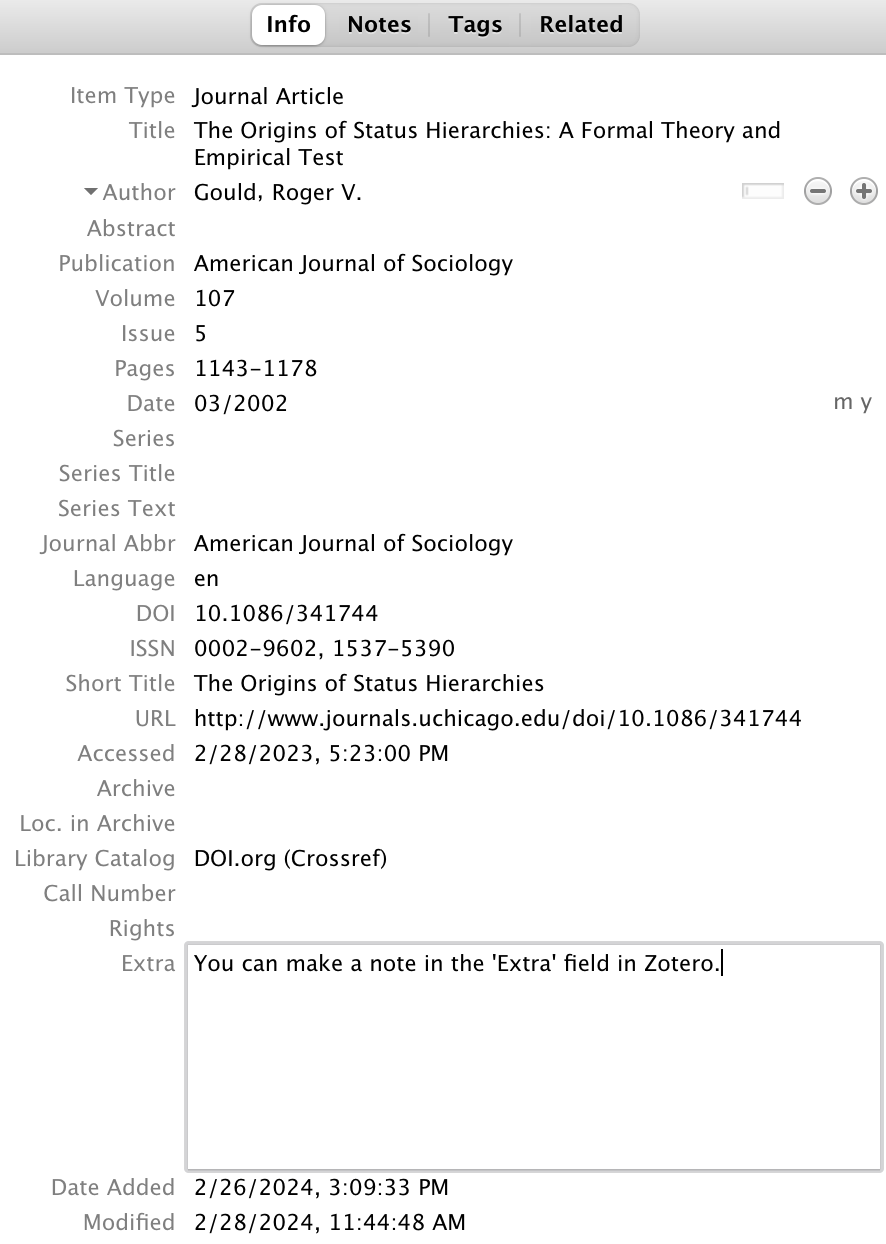
\includegraphics[width=0.5\textwidth]{screenshots/Zotero1a.png}
\caption{Example of the `Extra' field in Zotero}
\end{figure}

\begin{figure}[!ht]
\centering
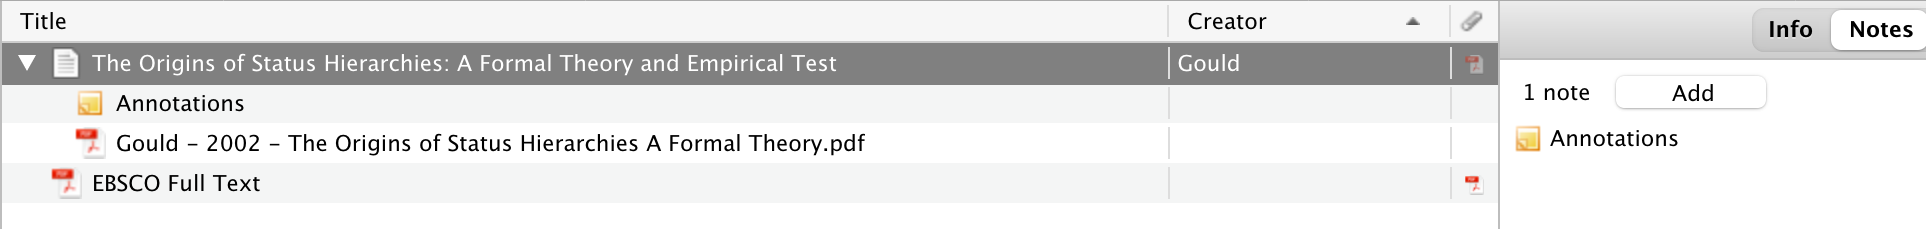
\includegraphics[width=\textwidth]{screenshots/Zotero1b.png}
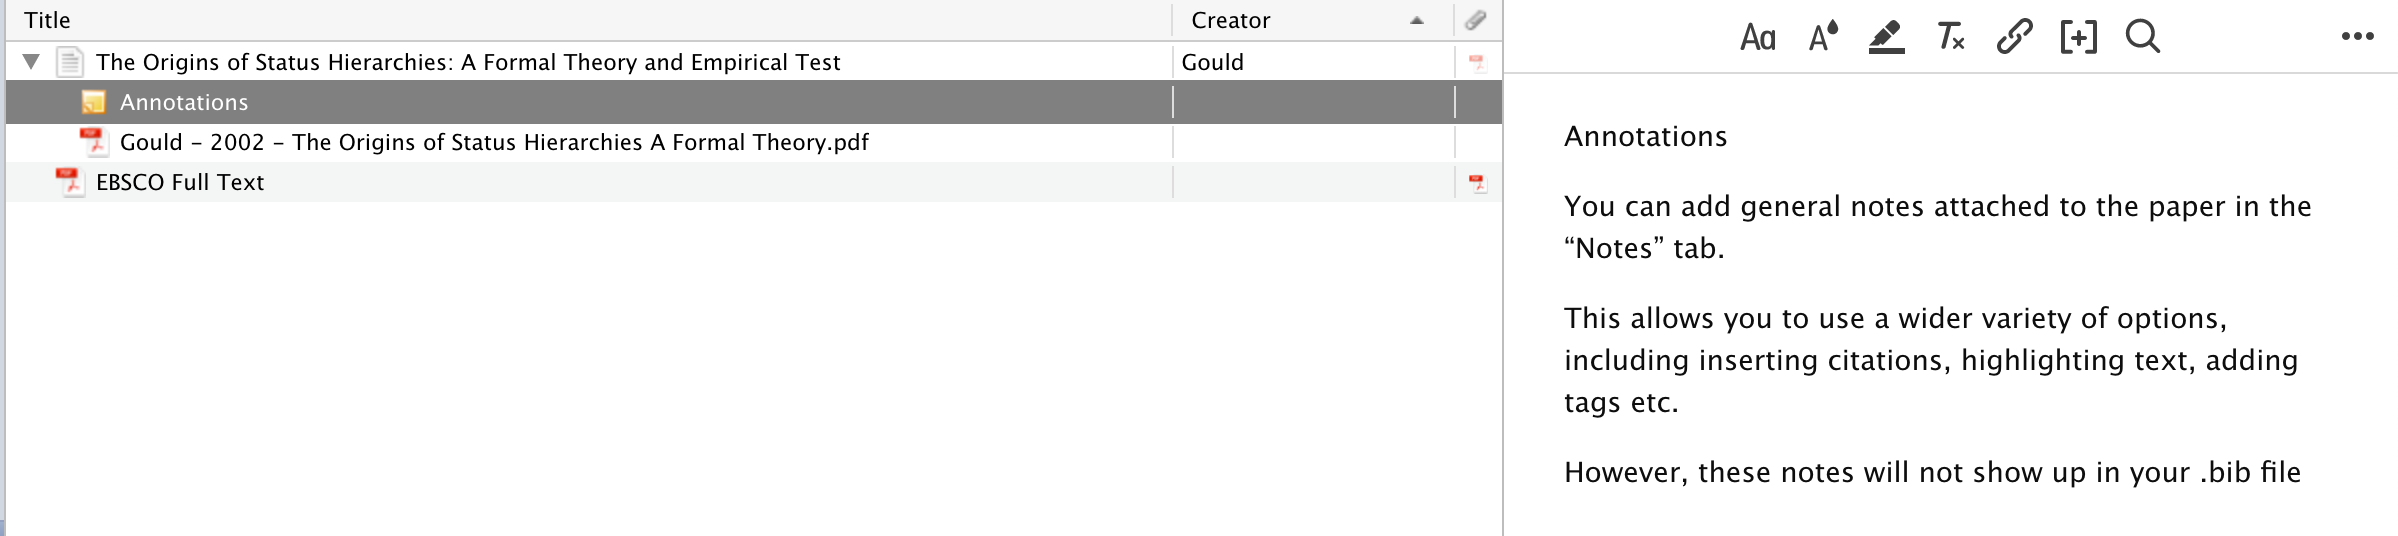
\includegraphics[width=\textwidth]{screenshots/Zotero1c.png}
\caption{Example of the `attached Note' in Zotero}
\end{figure}

The two function very differently. The `Extra' field will appear in the .bib file in the `note' field, and the `attached Note' will not. Furthermore, the attached Note is a lot more flexible in terms of formatting, and can even link to highlighted text in the file.

\begin{figure}[!ht]
\centering
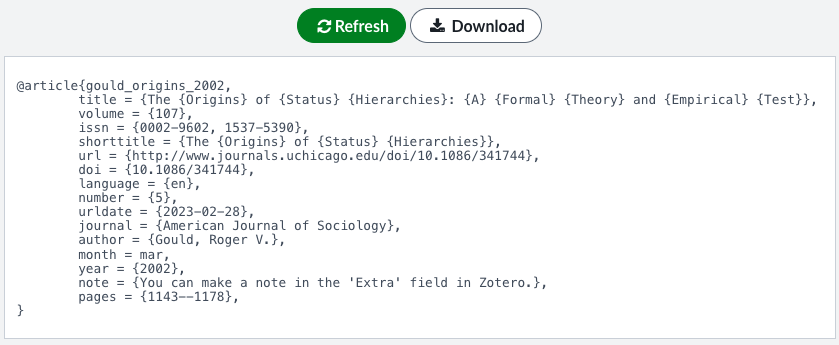
\includegraphics[width=\textwidth]{screenshots/Zotoero2.png}
\caption{The `Extra' field from Zotero appears as the `note' field in the synced .bib file}
\end{figure}



We \textbf{do not} recommend you use the ``Extra" field to create annotations, as the note field will be included when you print your bibliography. This field is better suited for relevant bibliographic information that you can't fit into any other fields in Zotero.

\begin{figure}[!ht]
\centering
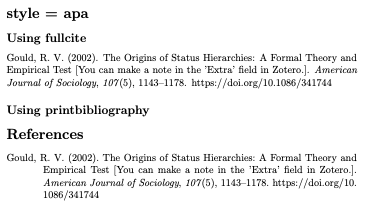
\includegraphics{screenshots/Zotero3b.png}
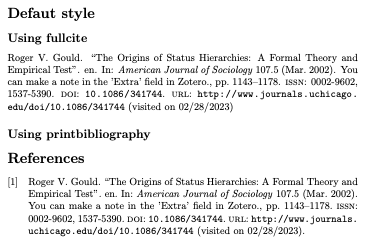
\includegraphics{screenshots/Zotero3c.png}
\caption{The `Extra' field from Zotero prints in both default and apa styles}
\end{figure}


Instead, it's probably the easiest if you keep your annotations as an attached note, and then copy-paste the contents of those into your annotated bibliography document. 

\FloatBarrier
\section*{Mendeley}
In general, there are two ways of creating notes in Mendeley, though if working in a Group library, you can only use one of those, as ``Notebooks" are, unfortunately unavailable. That said, in general, Notebooks are a great way of organizing your sources and quotes by topic and can be very helpful in building a literature review.

Your only option then is to use the ``General Notes`` in the Annotations tab. This functions pretty much like the ``Extra" field in Zotero and if you export the .bib file from Mendeley, what you include in the Annotations tab will show up in the ``note"  field. However, it seems that the Mendeley API does not export that field and therefore the field \textbf{will not appear} in your references on Overfleaf if you have it linked to Mendeley.

\begin{figure}[!ht]
\centering
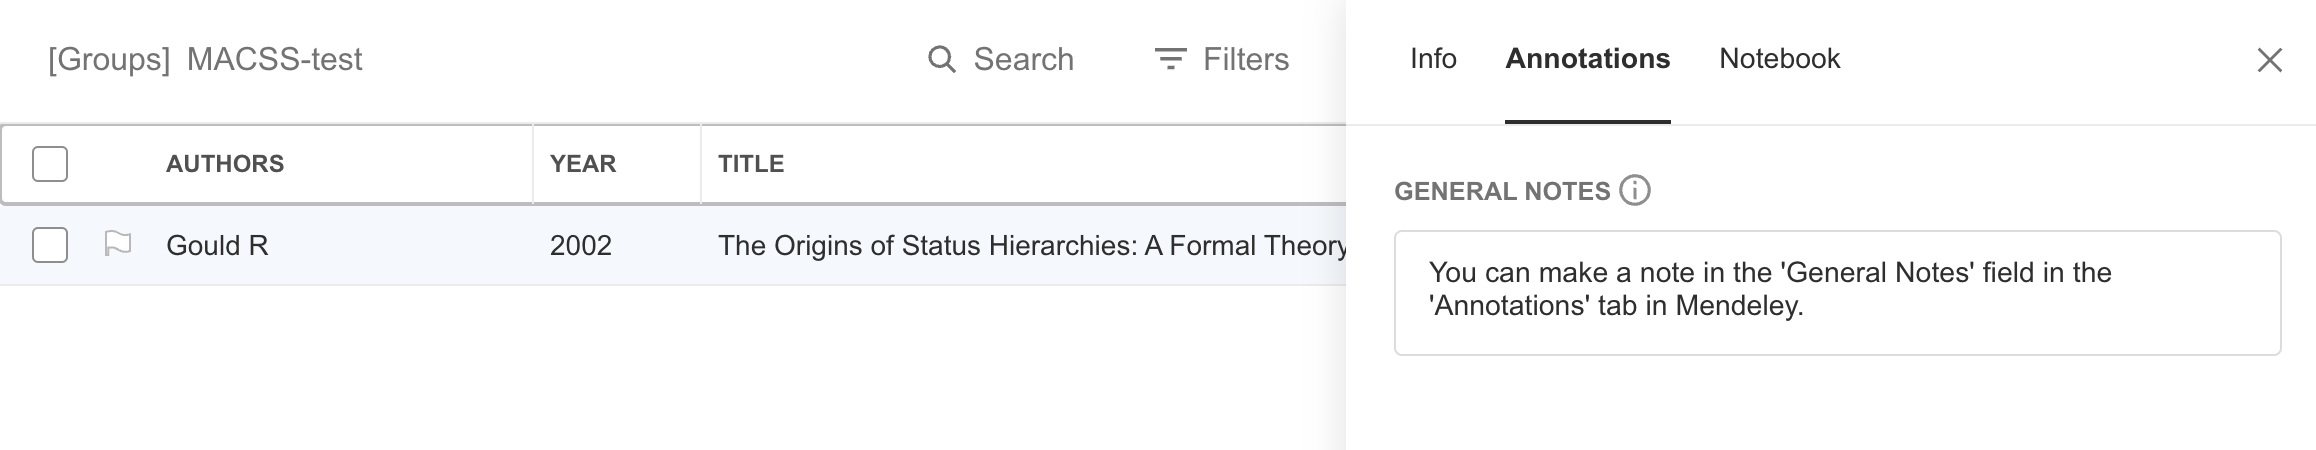
\includegraphics[width=\textwidth]{screenshots/Mendeley1a.png}
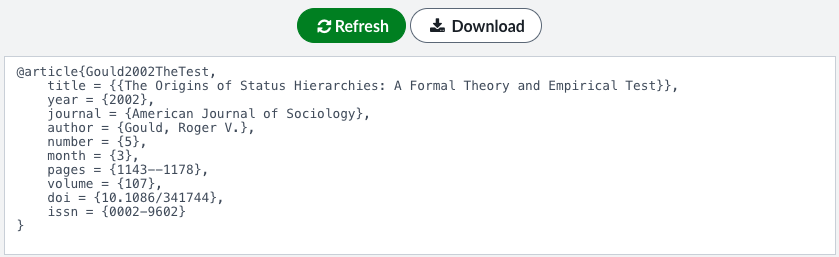
\includegraphics[width=\textwidth]{screenshots/Mendeley2.png}
\caption{the `Annotations' from Mendeley might not appear in a synced .bib file on Overleaf.}
\end{figure}


Without any additional info in the .bib file, your references will print normally, and you should simply use a combination of \verb|\fullcite{}| and copy-pasted annotations to compile your bibliography.

\begin{figure}[!ht]
\centering
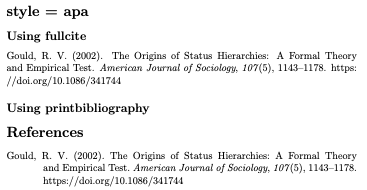
\includegraphics{screenshots/Mendeley3a.png}
\end{figure}

\FloatBarrier
\section*{.bib file}

Using a .bib file, you can take advantage of the field ``annote" which functions differently from the ``note" field in two important ways. First, it doesn't generally print when you print your bibliography (unless using a `non-standard' biblatex style, such as \textit{apa}). Second, using ``style=reading"  will print the annotation and label it as an annotation. This means that in order to compile the annotated bibliography from your .bib file, you simply have to change your style and you don't have to do any copy-pasting (make sure to format any text in the annotation in a LaTeX-friendly way, using escape characters when necessary).

\begin{figure}[!ht]
\centering
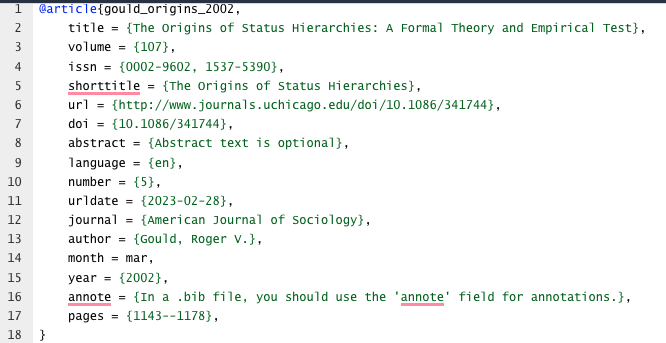
\includegraphics[width=\textwidth]{screenshots/Bib2.png}
\end{figure}

\begin{figure}[!ht]
\centering
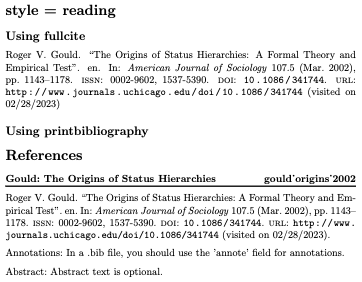
\includegraphics{screenshots/Bib3a.png}
\caption{Using the reading style and printing your bibliography will create your annotated bibliography for you}
\end{figure}

\begin{figure}[!ht]
\centering
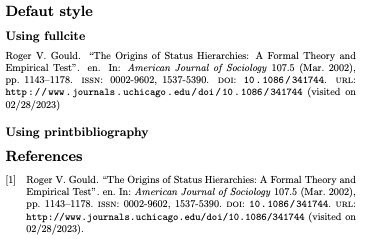
\includegraphics{screenshots/Bib3c.png}
\caption{biblatex styles, such as the default/non-specified style, do not print the annotations in the bibliography.}
\end{figure}


\begin{figure}[!ht]
\centering
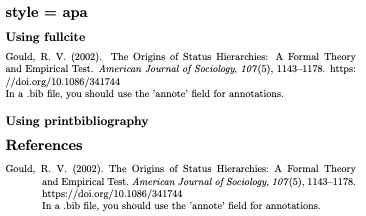
\includegraphics{screenshots/Bib3b.png}
\caption{However, apa style does include the annotation in the bibliography, so you should avoid it if you have information in the `annote' field, or you have to write a bit more code to suppress the field. The abstract field is suppressed}
\end{figure}

\end{document}

